\section{\trLimit{}与\trColimit{}}
\label{sec:limits-and-colimits}

在本节中，我们将给出∞-\trCategories{}中图表的（余）\trLimit{}的一种定义——它由%
\trKrause{}（A. Krause）与\trNikolaus{}（Thomas Nikolaus）向我们建议——并将它与通常的（余）%
\trLimit{}概念，即借助某些\trSliceCategory{}的\trInitialObject{}与%
\trTerminalObject{}来表述的那一概念，联系起来。我们将证明，（余）\trLimit{}若存在，
则在相差一个\trContractible{}选择空间的意义下唯一；并表明：一个∞-\trCategory{}%
容许小（余）\trLimit{}，当且仅当它分别容许小\trProduct{}与\trPullback{}、%
小\trCoproduct{}与\trPushout{}。随后，我们将
利用这些结果来指示：可以如何证明由空间组成的∞-\trCategory{}%
$\mathrm{Spc}$与由∞-\trCategories{}组成的∞-\trCategory{}%
$\mathrm{Cat}_{\infty}$具有全部小\trLimit{}与小\trColimit{}。我们将以选编的若干条
（余）\trLimit{}所具有的性质来结束本节。

下述\trColimit{}的定义取自\trKrause{}–\trNikolaus{}。

\begin{definition}\label{def:map-cone-space}
设 $F\colon K \to \C$ 是一个\trFunctor{}，并设 $x$ 是 $\C$ 的一个\trObject{}。我们用%
\trPullback{}%
\begin{center}
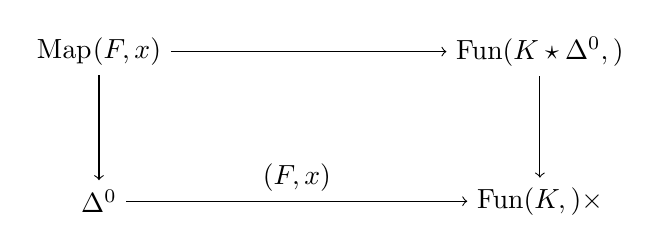
\begin{tikzpicture}
  \node (m) at (0,0) {$\mathrm{Map}_{\C}(F, x)$};
  \node (f) at (5.6,0) {$\mathrm{Fun}(K \star \Delta^0, \C)$};
  \node (d) at (0,-1.9) {$\Delta^0$};
  \node (g) at (5.6,-1.9) {$\mathrm{Fun}(K, \C) \times \C$};
  \draw[->] (m) -- (f);
  \draw[->] (m) -- (d);
  \draw[->] (f) -- (g);
  \draw[->] (d) -- node[above] {$(F, x)$} (g);
\end{tikzpicture}
\end{center}
来定义一个\trSimplicialSet{} $\mathrm{Map}_{\C}(F, x)$，其中右边的竖直映射由沿典范
包含 $K \cup \{\infty\} \subseteq K \star \Delta^0$ 的限制给出。
\end{definition}

\begin{lemma}\label{lem:map-cone-kan}
在上述情形中，$\mathrm{Map}_{\C}(F, x)$ 是一个\trInfinityGroupoid{}。若
$F = y\colon \Delta^0 \to \C$，则
$\mathrm{Map}_{\C}(y, x) = \mathrm{map}_{\C}(y, x)$。
\end{lemma}

\begin{proof}
沿\trMonomorphism{}的限制是一个\trConservative{}\trInnerFibration{}，而后者在%
\trPullback{}下稳定。第二部分由定义显然，因为 $\Delta^0 \star \Delta^0 = \Delta^1$。
\end{proof}

\begin{proposition}\label{prop:map-right-anodyne-homotopy}
设 $F\colon K \to \C$ 是一个\trFunctor{}，并设 $i\colon L \to K$ 是\trSimplicialSets{}%
的一个映射。那么，对 $\C$ 的一切\trObject{} $x$，$i$ 诱导出一个映射
$\mathrm{Map}_{\C}(F, x) \to \mathrm{Map}_{\C}(Fi, x)$。若 $i$ 是\trRightAnodyne{}的，
则该映射是一个\trHomotopyEquivalence{}。
\end{proposition}

\begin{proof}
为证明第一条陈述，我们观察到：存在一个交换图表
\begin{center}
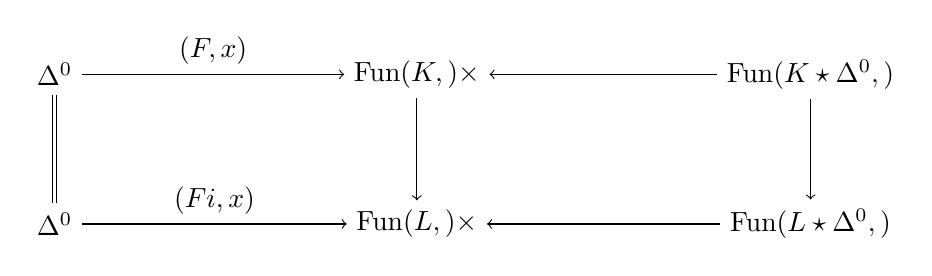
\begin{tikzpicture}
  \node (dt) at (0,0) {$\Delta^0$};
  \node (fk) at (4.6,0) {$\mathrm{Fun}(K, \C) \times \C$};
  \node (fsk) at (9.6,0) {$\mathrm{Fun}(K \star \Delta^0, \C)$};
  \node (db) at (0,-1.9) {$\Delta^0$};
  \node (fl) at (4.6,-1.9) {$\mathrm{Fun}(L, \C) \times \C$};
  \node (fsl) at (9.6,-1.9) {$\mathrm{Fun}(L \star \Delta^0, \C)$};
  \draw[->] (dt) -- node[above] {$(F, x)$} (fk);
  \draw[<-] (fk) -- (fsk);
  \draw[->] (db) -- node[above] {$(Fi, x)$} (fl);
  \draw[<-] (fl) -- (fsl);
  \draw[double, double distance=1.2pt] (dt) -- (db);
  \draw[->] (fk) -- (fl);
  \draw[->] (fsk) -- (fsl);
\end{tikzpicture}
\end{center}
它在诸\trPullback{}上诱导出我们所关心的那个映射。为了证明：当 $i$ 是%
\trRightAnodyne{}的时，该映射是\trHomotopyEquivalence{}，我们断言图表
\begin{center}
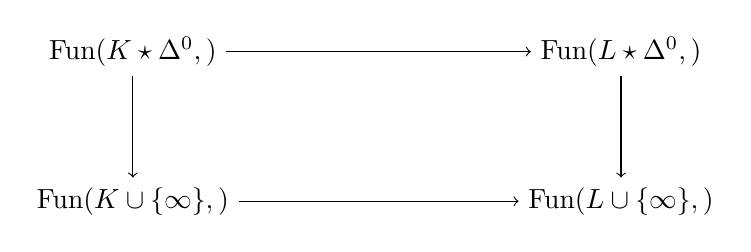
\begin{tikzpicture}
  \node (k) at (0,0) {$\mathrm{Fun}(K \star \Delta^0, \C)$};
  \node (l) at (6.2,0) {$\mathrm{Fun}(L \star \Delta^0, \C)$};
  \node (ku) at (0,-1.9) {$\mathrm{Fun}(K \cup \{\infty\}, \C)$};
  \node (lu) at (6.2,-1.9) {$\mathrm{Fun}(L \cup \{\infty\}, \C)$};
  \draw[->] (k) -- (l);
  \draw[->] (k) -- (ku);
  \draw[->] (l) -- (lu);
  \draw[->] (ku) -- (lu);
\end{tikzpicture}
\end{center}
是\trHomotopyCartesian{}。这可以通过计算由
\[
\mathrm{Fun}(L \star \Delta^0 \amalg_{L \cup \{\infty\}} K \cup \{\infty\}, \C)
\]
给出的\trPullback{}看出。而比较映射则由典范包含
\[
L \star \Delta^0 \amalg_{L \cup \{\infty\}} K \cup \{\infty\}
  \longrightarrow K \star \Delta^0
\]
诱导；由第 1 章中的\cref{lem:join-box-anodyne}，它是\trInnerAnodyne{}的，因为
$L \to K$ 是\trRightAnodyne{}的。因此，比较映射如所需是一个\trJoyalEquivalence{}。
由此可知，图表
\begin{center}
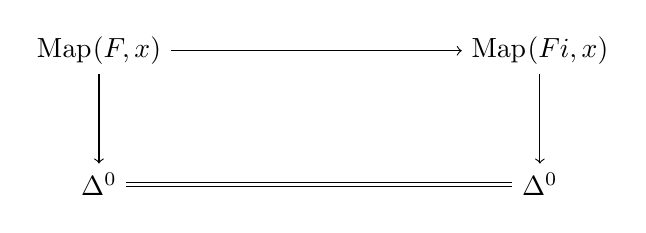
\begin{tikzpicture}
  \node (m) at (0,0) {$\mathrm{Map}_{\C}(F, x)$};
  \node (mi) at (5.6,0) {$\mathrm{Map}_{\C}(Fi, x)$};
  \node (d1) at (0,-1.7) {$\Delta^0$};
  \node (d2) at (5.6,-1.7) {$\Delta^0$};
  \draw[->] (m) -- (mi);
  \draw[->] (m) -- (d1);
  \draw[->] (mi) -- (d2);
  \draw[double, double distance=1.2pt] (d1) -- (d2);
\end{tikzpicture}
\end{center}
也是\trHomotopyCartesian{}，从而上方的映射如所期望的那样是一个%
\trHomotopyEquivalence{}。
\end{proof}

\begin{definition}\label{def:colimit-cone}
设 $F\colon K \to \C$ 是一个\trFunctor{}，并设 $\bar{F}\colon K \star \Delta^0 \to \C$
是 $F$ 之上的一个\trCone{}。我们称 $\bar{F}$ 是一个\emph{\trColimit{}\trCone{}}（colimit
cone），如果对 $\C$ 的一切\trObject{} $x$，典范映射
\[
\mathrm{Map}_{\C}(\bar{F}, x) \longrightarrow \mathrm{Map}_{\C}(F, x)
\]
是一个\trHomotopyEquivalence{}。
\end{definition}

\begin{remark}\label{rem:colimit-cone-criterion}
由于映射 $\{\infty\} \to K \star \Delta^0$ 是\trRightAnodyne{}的，我们发现：对任意%
\trCone{} $\bar{F}\colon K \star \Delta^0 \to \C$，典范映射
\[
\mathrm{Map}_{\C}(\bar{F}, x) \longrightarrow
  \mathrm{Map}_{\C}(\bar{F}(\infty), x)
  = \mathrm{map}_{\C}(\bar{F}(\infty), x)
\]
是一个\trHomotopyEquivalence{}。于是，$\bar{F}$ 是一个\trColimit{}\trCone{}，当且仅当对
$\C$ 的一切\trObject{} $x$，上述诸映射拼合成一个\trHomotopyEquivalence{}%
\[
\mathrm{Map}_{\C}(F, x) \simeq \mathrm{map}_{\C}(\bar{F}(\infty), x).
\]
\end{remark}

\begin{definition}\label{def:limit-cocone}
对偶地，对一个\trFunctor{} $F\colon K \to \C$，我们把\trSimplicialSet{}%
$\mathrm{Map}_{\C}(x, F)$ 定义为\trPullback{}%
\begin{center}
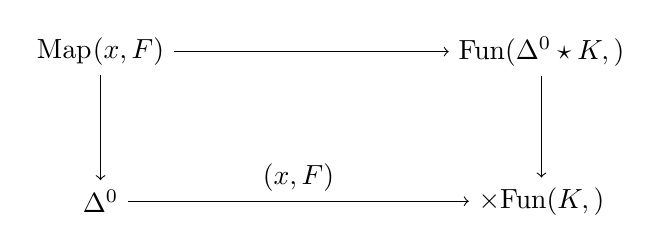
\begin{tikzpicture}
  \node (m) at (0,0) {$\mathrm{Map}_{\C}(x, F)$};
  \node (f) at (5.6,0) {$\mathrm{Fun}(\Delta^0 \star K, \C)$};
  \node (d) at (0,-1.9) {$\Delta^0$};
  \node (g) at (5.6,-1.9) {$\C \times \mathrm{Fun}(K, \C)$};
  \draw[->] (m) -- (f);
  \draw[->] (m) -- (d);
  \draw[->] (f) -- (g);
  \draw[->] (d) -- node[above] {$(x, F)$} (g);
\end{tikzpicture}
\end{center}
与前面一样，映射 $i\colon L \to K$ 诱导出一个映射
$\mathrm{Map}_{\C}(x, F) \to \mathrm{Map}_{\C}(x, Fi)$，当 $i$ 是\trLeftAnodyne{}的
时，它是\trHomotopyEquivalence{}。于是，$F$ 的一个\trCocone{}%
$\bar{F}\colon \Delta^0 \star K \to \C$ 称为一个\emph{\trLimit{}\trCocone{}}（limit
cocone），如果典范映射
\[
\mathrm{Map}_{\C}(x, \bar{F}) \longrightarrow \mathrm{Map}_{\C}(x, F)
\]
对 $\C$ 中的一切 $x$ 都是\trHomotopyEquivalence{}。
\end{definition}

\begin{remark}\label{rem:initial-terminal-as-colimits}
让我们将这个定义与\trInitialObject{}与\trTerminalObject{}的定义比较一番。目标是
看出：一个\trInitialObject{}恰是空\trFunctor{} $\varnothing \to \C$ 的一个%
\trColimit{}：空\trFunctor{}之上的一个\trCone{}无非就是一个\trFunctor{}%
$y\colon \Delta^0 \to \C$。此外，$\mathrm{Map}_{\C}(\varnothing, x) \cong \Delta^0$，
而由\cref{lem:map-cone-kan}，$\mathrm{Map}_{\C}(y, x) = \mathrm{map}_{\C}(y, x)$。
于是我们发现：一个\trObject{} $y$（视为空\trFunctor{}之上的一个\trCone{}）是一个%
\trColimit{}\trCone{}，当且仅当对一切\trObject{} $x$，\trMappingSpace{}%
$\mathrm{map}_{\C}(y, x)$ 与 $\Delta^0$ 成\trJoyalEquivalence{}，亦即是%
\trContractible{}。因此，空\trFunctor{}之上的一个\trColimit{}\trCone{}恰好就是一个%
\trInitialObject{}。同样地，空\trFunctor{}之上的一个\trLimit{}\trCocone{}恰好就是一个%
\trTerminalObject{}。
\end{remark}

\begin{example*}
在一个集合（视为一个\trDiscreteCategory{}）上取的\trColimit{}称为\emph{\trCoproduct{}}（coproduct）。
在一个集合上取的\trLimit{}称为\emph{\trProduct{}}（product）。
\end{example*}

\begin{example*}
$\Lambda^2_0 \to \C$ 的\trColimit{}称为\emph{\trPushout{}}（pushout）。
$\Lambda^2_2 \to \C$ 的\trLimit{}称为\emph{\trPullback{}}（pullback）。注意
$\Lambda^2_0 \star \Delta^0 \cong \Delta^1 \times \Delta^1$，同样地
$\Delta^0 \star \Lambda^2_2 \cong \Delta^1 \times \Delta^1$。
\end{example*}

在\cref{lem:terminal-characterizations}中，我们把\trInitialObject{}与%
\trTerminalObject{}刻画为如下性质：某些\trSlice{}之间的映射是%
\trTrivialFibration{}。现在，
我们将朝着对一般\trColimit{}与\trLimit{}的类似描述前进。作为开端，我们有下述引理。

\begin{lemma}\label{lem:fat-join-iso}
对任意两个\trSimplicialSets{} $K$ 与 $S$，存在一个典范同构
\[
K \diamond S \cong \bigl[(K \diamond \Delta^0) \times S\bigr]
  \amalg_{K \times S} K,
\]
它与来自 $K$ 与 $S$ 的映射相容。
\end{lemma}

\begin{proof}
考虑图表
\begin{center}
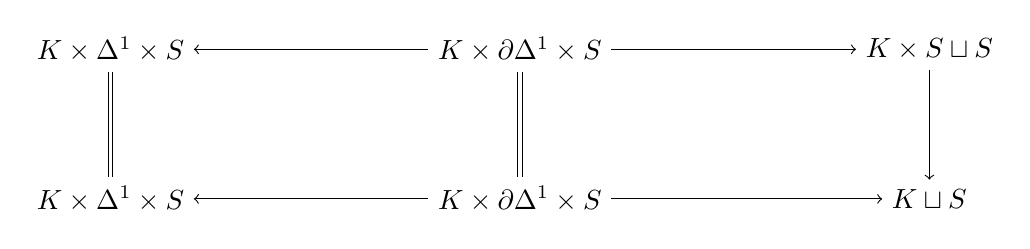
\begin{tikzpicture}
  \node (a) at (0,0) {$K \times \Delta^1 \times S$};
  \node (b) at (5.2,0) {$K \times \partial\Delta^1 \times S$};
  \node (c) at (10.4,0) {$K \times S \sqcup S$};
  \node (a2) at (0,-1.9) {$K \times \Delta^1 \times S$};
  \node (b2) at (5.2,-1.9) {$K \times \partial\Delta^1 \times S$};
  \node (c2) at (10.4,-1.9) {$K \sqcup S$};
  \draw[<-] (a) -- (b);
  \draw[->] (b) -- (c);
  \draw[<-] (a2) -- (b2);
  \draw[->] (b2) -- (c2);
  \draw[double, double distance=1.2pt] (a) -- (a2);
  \draw[double, double distance=1.2pt] (b) -- (b2);
  \draw[->] (c) -- (c2);
\end{tikzpicture}
\end{center}
其两个\trPushout{}分别由 $(K \diamond \Delta^0) \times S$ 与 $K \diamond S$ 给出。
于是我们发现，在下述图表中右边那个小方块是一个\trPushout{}：
\begin{center}
\begin{tikzpicture}
  \node (a) at (0,0) {$K \times S$};
  \node (b) at (4.8,0) {$K \times S \sqcup S$};
  \node (c) at (9.4,0) {$(K \diamond \Delta^0) \times S$};
  \node (a2) at (0,-1.9) {$K$};
  \node (b2) at (4.8,-1.9) {$K \sqcup S$};
  \node (c2) at (9.4,-1.9) {$K \diamond S$};
  \draw[->] (a) -- (b);
  \draw[->] (b) -- (c);
  \draw[->] (a2) -- (b2);
  \draw[->] (b2) -- (c2);
  \draw[->] (a) -- (a2);
  \draw[->] (b) -- (b2);
  \draw[->] (c) -- (c2);
\end{tikzpicture}
\end{center}
左边的方块一目了然是一个\trPushout{}，故拼合起来的方块也是一个\trPushout{}。
\end{proof}

\begin{lemma}\label{lem:map-slice-homotopy-cartesian}
设 $F\colon K \to \C$ 是一个\trFunctor{}，并设 $x$ 是 $\C$ 的一个\trObject{}。那么图表
\begin{center}
\begin{tikzpicture}
  \node (m1) at (0,0) {$\mathrm{Map}_{\C}(F, x)$};
  \node (s1) at (3.8,0) {$\C_{F/}$};
  \node (d1) at (0,-1.9) {$\Delta^0$};
  \node (c1) at (3.8,-1.9) {$\C$};
  \node (m2) at (6.6,0) {$\mathrm{Map}_{\C}(x, F)$};
  \node (s2) at (10.4,0) {$\C_{/F}$};
  \node (d2) at (6.6,-1.9) {$\Delta^0$};
  \node (c2) at (10.4,-1.9) {$\C$};
  \draw[->] (m1) -- (s1);
  \draw[->] (m1) -- (d1);
  \draw[->] (s1) -- (c1);
  \draw[->] (d1) -- node[above] {$x$} (c1);
  \draw[->] (m2) -- (s2);
  \draw[->] (m2) -- (d2);
  \draw[->] (s2) -- (c2);
  \draw[->] (d2) -- node[above] {$x$} (c2);
\end{tikzpicture}
\end{center}
是\trHomotopyCartesian{}。
\end{lemma}

\begin{proof}
我们对左边的方块论证，另一种情形是类似的。我们首先证明：存在一个\trPullback{}图表
\begin{center}
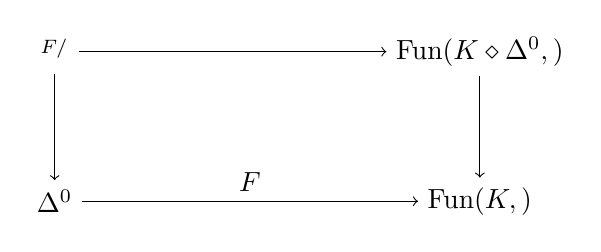
\begin{tikzpicture}
  \node (cf) at (0,0) {$\C^{F/}$};
  \node (fu) at (5.4,0) {$\mathrm{Fun}(K \diamond \Delta^0, \C)$};
  \node (d) at (0,-1.9) {$\Delta^0$};
  \node (fk) at (5.4,-1.9) {$\mathrm{Fun}(K, \C)$};
  \draw[->] (cf) -- (fu);
  \draw[->] (cf) -- (d);
  \draw[->] (fu) -- (fk);
  \draw[->] (d) -- node[above] {$F$} (fk);
\end{tikzpicture}
\end{center}
暂时姑且把这个\trPullback{}称为 $\Phi(F)$。对一个\trSimplicialSet{} $S$ 而言，到
$\C^{F/}$ 的一个映射对应于一个映射 $K \diamond S \to \C$，而到 $\Phi(F)$ 的一个映射
则对应于一个映射
\[
(K \diamond \Delta^0) \times S \amalg_{K \times S} K \longrightarrow \C.
\]
于是，借助\cref{lem:fat-join-iso}，我们便给证明的第一部分收尾。

接下来，我们用\trPullback{}%
\begin{center}
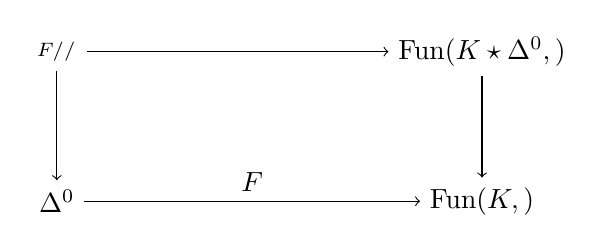
\begin{tikzpicture}
  \node (cf) at (0,0) {$\C_{F//}$};
  \node (fu) at (5.4,0) {$\mathrm{Fun}(K \star \Delta^0, \C)$};
  \node (d) at (0,-1.9) {$\Delta^0$};
  \node (fk) at (5.4,-1.9) {$\mathrm{Fun}(K, \C)$};
  \draw[->] (cf) -- (fu);
  \draw[->] (cf) -- (d);
  \draw[->] (fu) -- (fk);
  \draw[->] (d) -- node[above] {$F$} (fk);
\end{tikzpicture}
\end{center}
定义一个\trSimplicialSet{} $\C_{F//}$。由典范映射
$K \diamond \Delta^0 \to K \star \Delta^0$，我们得到映射
\[
\C_{F//} \longrightarrow \C^{F/} \longleftarrow \C_{F/},
\]
我们断言两者都是\trJoyalEquivalence{}：右边的映射已在第 2 章中的%
\cref{prop:slice-fat-slice-joyal-equivalence}中处理过；而左边的映射，则再次由如下
事实得出：映射 $K \diamond \Delta^0 \to K \star \Delta^0$ 是一个%
\trJoyalEquivalence{}，并且由第 2 章中的\cref{lem:pullback-joyal-equivalence}，
涉及 $\C^{F/}$ 与 $\C_{F//}$ 的那些\trPullback{}在\trJoyalEquivalence{}下不变。
随后我们考虑图表
\begin{center}
\begin{tikzpicture}
  \node (m) at (0,0) {$\mathrm{Map}_{\C}(F, x)$};
  \node (cff) at (3.8,0) {$\C_{F//}$};
  \node (fsk) at (8.0,0) {$\mathrm{Fun}(K \star \Delta^0, \C)$};
  \node (d0) at (0,-2.0) {$\Delta^0$};
  \node (c) at (3.8,-2.0) {$\C$};
  \node (fkc) at (8.0,-2.0) {$\mathrm{Fun}(K, \C) \times \C$};
  \node (d1) at (3.8,-4.0) {$\Delta^0$};
  \node (fk) at (8.0,-4.0) {$\mathrm{Fun}(K, \C)$};
  \draw[->] (m) -- (cff);
  \draw[->] (cff) -- (fsk);
  \draw[->] (m) -- (d0);
  \draw[->] (cff) -- (c);
  \draw[->] (fsk) -- (fkc);
  \draw[->] (d0) -- (c);
  \draw[->] (c) -- (fkc);
  \draw[->] (c) -- (d1);
  \draw[->] (fkc) -- (fk);
  \draw[->] (d1) -- (fk);
\end{tikzpicture}
\end{center}
它由若干个\trPullback{}图表组成。于是，断言由存在\trJoyalEquivalence{}%
$\C_{F//} \simeq \C^{F/}$ 这一事实得出。
\end{proof}

\begin{remark}\label{rem:fat-join-variant}
我们本可以定义 $\mathrm{Map}_{\C}(F, x)$ 的一个变体，其做法是用\trFatJoin{}代替
通常的\trJoin{}。这样得到的∞-\trGroupoid{} $\widetilde{\mathrm{Map}}_{\C}(F, x)$
典范地等价于 $\mathrm{Map}_{\C}(F, x)$，并且在有用的场合我们将随意地交换使用两者。
\cref{lem:map-slice-homotopy-cartesian}的证明随即便表明：对这个变体而言，下述图表
是一个\trPullback{}：
\begin{center}
\begin{tikzpicture}
  \node (m) at (0,0) {$\widetilde{\mathrm{Map}}_{\C}(F, x)$};
  \node (cf) at (4.4,0) {$\C^{F/}$};
  \node (d) at (0,-1.9) {$\Delta^0$};
  \node (c) at (4.4,-1.9) {$\C$};
  \draw[->] (m) -- (cf);
  \draw[->] (m) -- (d);
  \draw[->] (cf) -- (c);
  \draw[->] (d) -- (c);
\end{tikzpicture}
\end{center}
\end{remark}

下述定理表明，我们的\trLimit{}与\trColimit{}定义与通常给出的定义相一致，例如在
\cite{Lur09} 中给出的那个定义。

\begin{theorem}\label{thm:colimit-cone-initial}
设 $F\colon K \to \C$ 是∞-\trCategory{} $\C$ 中的一个图表。$F$ 的一个\trCone{}%
$\bar{F}\colon K \star \Delta^0 \to \C$ 是一个\trColimit{}\trCone{}，当且仅当它是
$\C_{F/}$ 的一个\trInitialObject{}。对偶地，$F$ 的一个\trCocone{}%
$\bar{F}\colon \Delta^0 \star K \to \C$ 是一个\trLimit{}\trCocone{}，当且仅当它是
$\C_{/F}$ 的一个\trTerminalObject{}。
\end{theorem}

\begin{proof}
一个\trCocone{} $\bar{F}$ 给出一个交换图表\footnote{译注：原书作
「cocone（余锥）」，疑为 cone（锥）之误。——译者注}
\begin{center}
\begin{tikzpicture}
  \node (a) at (0,0) {$\C_{\bar{F}/}$};
  \node (b) at (4.4,0) {$\C_{F/}$};
  \node (c) at (2.2,-2.2) {$\C$};
  \draw[->] (a) -- (b);
  \draw[->] (a) -- (c);
  \draw[->] (b) -- (c);
\end{tikzpicture}
\end{center}
它由若干个\trLeftFibration{}组成。由\cref{ex:slice-iso-adjoint}，$\bar{F}$ 是一个\trInitialObject{}，
当且仅当水平映射是一个\trTrivialFibration{}；而这又当且仅当它是一个%
\trJoyalEquivalence{}。由第 3 章中的\cref{thm:fibrewise-criterion}，情形正是如此：
它当且仅当在 $\C$ 的诸\trObject{} $x$ 上的\trFibre{}之间诱导出的映射是%
\trHomotopyEquivalence{}。由\cref{lem:map-slice-homotopy-cartesian}，诸\trFibre{}上
诱导出的映射等价于映射
\[
\mathrm{Map}_{\C}(\bar{F}, x) \longrightarrow \mathrm{Map}_{\C}(F, x).
\]
于是我们发现：映射 $\C_{\bar{F}/} \to \C_{F/}$ 是一个\trJoyalEquivalence{}，当且仅当
$\bar{F}$ 是 $F$ 的一个\trColimit{}\trCone{}。关于\trLimit{}的论证是一样的，只需使用%
\cref{lem:map-slice-homotopy-cartesian}的对偶版本。
\end{proof}

下述结果对我们后面的目的将会非常有用。

\begin{proposition}\label{prop:pushout-map-homotopy-cartesian}
设 $\C$ 是一个∞-\trCategory{}，并考虑\trSimplicialSets{}的一个\trPushout{}%
\begin{center}
\begin{tikzpicture}
  \node (a) at (0,0) {$A$};
  \node (b) at (2.8,0) {$B$};
  \node (c) at (0,-1.9) {$C$};
  \node (k) at (2.8,-1.9) {$K$};
  \draw[->] (a) -- node[above] {$i$} (b);
  \draw[->] (a) -- (c);
  \draw[->] (b) -- (k);
  \draw[->] (c) -- (k);
\end{tikzpicture}
\end{center}
其中映射 $i$ 是一个\trMonomorphism{}。设 $F\colon K \to \C$ 是一个\trFunctor{}，并把
$F$ 到 $A$、$B$ 与 $C$ 上的限制分别记作 $F_A$、$F_B$ 与 $F_C$。那么，对 $\C$ 的每个%
\trObject{} $x$，图表
\begin{center}
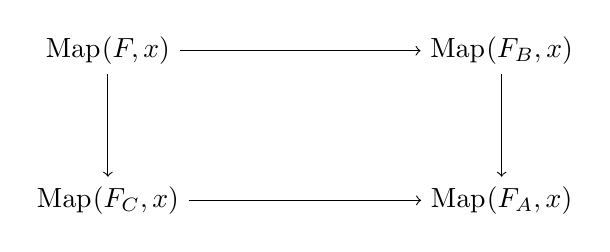
\begin{tikzpicture}
  \node (m) at (0,0) {$\mathrm{Map}_{\C}(F, x)$};
  \node (mb) at (5.0,0) {$\mathrm{Map}_{\C}(F_B, x)$};
  \node (mc) at (0,-1.9) {$\mathrm{Map}_{\C}(F_C, x)$};
  \node (ma) at (5.0,-1.9) {$\mathrm{Map}_{\C}(F_A, x)$};
  \draw[->] (m) -- (mb);
  \draw[->] (m) -- (mc);
  \draw[->] (mb) -- (ma);
  \draw[->] (mc) -- (ma);
\end{tikzpicture}
\end{center}
是\trHomotopyCartesian{}。
\end{proposition}

\begin{proof}
我们可以把 $\mathrm{Map}_{\C}(F, x)$ 替换成
$\widetilde{\mathrm{Map}}_{\C}(F, x)$，即使用\trFatSlice{}的那个版本。首先，我们
观察到该图表是一个\trPullback{}：这是因为
$\widetilde{\mathrm{Map}}_{\C}(F, x)$ 被定义为一个\trFibre{}，而\trFibre{}与%
\trPullback{}交换，并且\trFunctor{} $\mathrm{Fun}(-, \C)$ 与
$\mathrm{Fun}(-, \C) \times \C$ 两者都把\trPushout{}送到\trPullback{}。然后，我们
可以利用 $- \diamond \Delta^0$ 也保持\trPushout{}这一事实。因此，只需证明映射
$\widetilde{\mathrm{Map}}_{\C}(F_B, x) \to \widetilde{\mathrm{Map}}_{\C}(F_A, x)$
是一个\trKanFibration{}。由\cref{rem:fat-join-variant}，存在一个\trPullback{}图表
\begin{center}
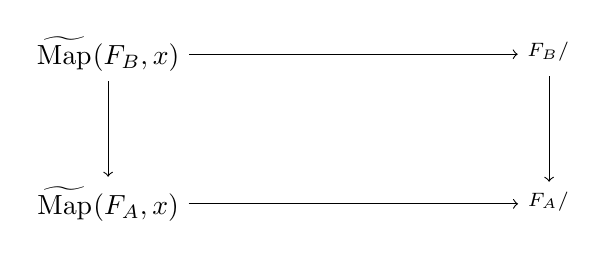
\begin{tikzpicture}
  \node (mb) at (0,0) {$\widetilde{\mathrm{Map}}_{\C}(F_B, x)$};
  \node (cb) at (5.6,0) {$\C^{F_B/}$};
  \node (ma) at (0,-1.9) {$\widetilde{\mathrm{Map}}_{\C}(F_A, x)$};
  \node (ca) at (5.6,-1.9) {$\C^{F_A/}$};
  \draw[->] (mb) -- (cb);
  \draw[->] (mb) -- (ma);
  \draw[->] (cb) -- (ca);
  \draw[->] (ma) -- (ca);
\end{tikzpicture}
\end{center}
因此只需回忆起：映射 $\C^{F_B/} \to \C^{F_A/}$ 是一个\trLeftFibration{}，于是它的%
\trPullback{}是诸\trKanComplex{}之间的一个\trLeftFibration{}，进而是一个%
\trKanFibration{}。
\end{proof}

我们再次发现，（余）\trLimit{}若存在，则在相差一个\trContractible{}选择空间的
意义下唯一。

\begin{lemma}\label{lem:colim-cones-contractible}
设 $p\colon K \to \C$ 是一个图表。设
$(\C_{p/})^{\mathrm{colim}} \subseteq \C_{p/}$ 与
$(\C_{/p})^{\mathrm{lim}} \subseteq \C_{/p}$ 分别为由诸\trColimit{}\trCone{}与诸%
\trLimit{}\trCocone{}张成的满子范畴。那么 $(\C_{p/})^{\mathrm{colim}}$
与 $(\C_{/p})^{\mathrm{lim}}$ 要么为空，要么是\trContractible{}\trKanComplex{}。
\end{lemma}

\begin{proof}
这无非是\trInitialObject{}与\trTerminalObject{}情形的一个重新表述，见%
\cref{prop:terminal-contractible}。
\end{proof}

下述结果在后面当我们证明\trColimit{}的构成（若可能的话）是一个\trFunctor{}时
将会是必需的。

\begin{proposition}\label{prop:map-fun-mapping-space}
设 $K$ 是一个\trSimplicialSet{}，$F\colon K \to \C$ 是一个\trFunctor{}，而 $x$ 是
∞-\trCategory{} $\C$ 的一个\trObject{}。那么存在\trSimplicialSets{}的一个典范同构
\[
\widetilde{\mathrm{Map}}_{\C}(F, x) \cong
  \mathrm{map}_{\mathrm{Fun}(K, \C)}(F, \mathrm{const}_x),
\]
从而有典范\trHomotopyEquivalence{}%
\[
\mathrm{Map}_{\C}(F, x) \simeq
  \mathrm{map}_{\mathrm{Fun}(K, \C)}(F, \mathrm{const}_x).
\]
\end{proposition}

\begin{proof}
第二条断言由\cref{rem:fat-join-variant}中的典范\trHomotopyEquivalence{}%
$\mathrm{Map}_{\C}(F, x) \simeq \widetilde{\mathrm{Map}}_{\C}(F, x)$ 得出。为了看出
第一条断言，我们断言图表
\begin{center}
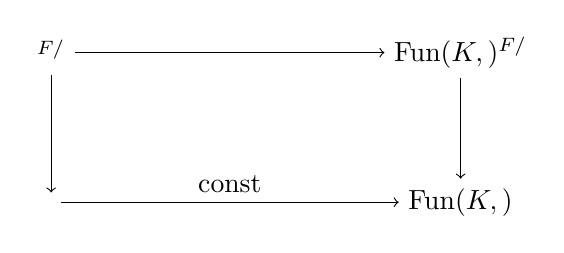
\begin{tikzpicture}
  \node (cf) at (0,0) {$\C^{F/}$};
  \node (ff) at (5.2,0) {$\mathrm{Fun}(K, \C)^{F/}$};
  \node (c) at (0,-1.9) {$\C$};
  \node (fk) at (5.2,-1.9) {$\mathrm{Fun}(K, \C)$};
  \draw[->] (cf) -- (ff);
  \draw[->] (cf) -- (c);
  \draw[->] (ff) -- (fk);
  \draw[->] (c) -- node[above] {$\mathrm{const}$} (fk);
\end{tikzpicture}
\end{center}
是笛卡尔的（cartesian），其中我们也将 $F$ 视为一个\trFunctor{}%
$\Delta^0 \to \mathrm{Fun}(K, \C)$。于是，在我们的断言成立这一假设下，沿一个映射
$x\colon \Delta^0 \to \C$ 取\trPullback{}，我们便得到一个同构
\[
\widetilde{\mathrm{Map}}_{\C}(F, x) \xrightarrow{\ \simeq\ }
  \mathrm{map}_{\mathrm{Fun}(K, \C)}(F, \mathrm{const}_x)
\]
如所期望。为了看出这个断言，注意到：一个映射 $X \to \C^{F/}$ 对应于一个映射
$X \diamond K \to \C$，后者到 $K$ 上的限制为 $F$。同样地，到上述图表的%
\trPullback{}的一个映射对应于一个映射
\[
(X \diamond \Delta^0) \times K \amalg_{X \times K} X \longrightarrow \C,
\]
其限制同样恰当。于是，断言再次由\cref{lem:fat-join-iso}得出。
\end{proof}

\begin{lemma}\label{lem:id-colimit-cone-terminal}
设 $\C$ 是一个∞-\trCategory{}，并设
$\bar{\mathrm{id}}\colon \C \star \Delta^0 \to \C$ 是 $\C$ 的恒同之上的一个%
\trCone{}。那么，$\bar{\mathrm{id}}$ 是一个\trColimit{}\trCone{}，当且仅当
$\bar{\mathrm{id}}(\infty)$ 是一个\trTerminalObject{}。
特别地，$\C$ 具有一个\trTerminalObject{}，当且仅当恒同\trFunctor{}容有一个%
\trColimit{}。
\end{lemma}

\begin{proof}
假设 $t$ 是 $\C$ 的一个\trTerminalObject{}。考虑复合 $\{t\} \to \C \to \C$，其中
后一个\trFunctor{}是恒同。我们便得到切片上诱导的一个\trFunctor{}%
$\C_{\mathrm{id}/} \to \C_{t/}$，它是一个\trTrivialFibration{}，因为由%
\cref{lem:initial-left-anodyne}，包含 $\{t\} \to \C$ 是\trRightAnodyne{}的。由于
$\C_{t/}$ 具有一个\trInitialObject{}，这对 $\C_{\mathrm{id}/}$ 也成立。于是，由%
\cref{thm:colimit-cone-initial}，$t$ 是恒同\trFunctor{}的一个\trColimit{}。反之，
让我们假设恒同\trFunctor{}容有一个\trColimit{}\trCone{} $\bar{\mathrm{id}}$。我们需要证明：
$x = \bar{\mathrm{id}}(\infty)$ 是一个\trTerminalObject{}。为此，我们将援引%
\cref{lem:terminal-characterizations}并考虑\trLiftingProblem{}%
\begin{center}
\begin{tikzpicture}
  \node (v) at (0,0) {$\Delta^{\{n\}}$};
  \node (bd) at (2.6,0) {$\partial\Delta^n$};
  \node (c) at (5.2,0) {$\C$};
  \node (dn) at (2.6,-1.8) {$\Delta^n$};
  \draw[->] (v) -- (bd);
  \draw[->] (bd) -- (c);
  \draw[->] (bd) -- (dn);
  \draw[->, dashed] (dn) -- (c);
  \draw[->, bend left=25] (v) to (c);
\end{tikzpicture}
\end{center}
其中上面的复合由\trObject{} $x$ 给出。对这个图表应用\trFunctor{} $- \star \Delta^0$，
我们便得到
\begin{center}
\begin{tikzpicture}
  \node (dn) at (0,0) {$\Delta^{\{n\}}$};
  \node (dnn) at (3.6,0) {$\Delta^{\{n,n+1\}}$};
  \node (bd) at (0,-2.2) {$\partial\Delta^n$};
  \node (lam) at (3.6,-2.2) {$\Lambda^{n+1}_{n+1}$};
  \node (cs) at (7.0,-2.2) {$\C \star \Delta^0$};
  \node (c) at (10.2,-2.2) {$\C$};
  \node (dn2) at (0,-4.4) {$\Delta^n$};
  \node (dnp) at (3.6,-4.4) {$\Delta^{n+1}$};
  \draw[->] (dn) -- (dnn);
  \draw[->] (dn) -- (bd);
  \draw[->] (dnn) -- (lam);
  \draw[->] (bd) -- (lam);
  \draw[->] (lam) -- (cs);
  \draw[->] (cs) -- node[above] {$\bar{\mathrm{id}}$} (c);
  \draw[->] (bd) -- (dn2);
  \draw[->] (lam) -- (dnp);
  \draw[->] (dn2) -- (dnp);
  \draw[->, bend left=20] (dnn) to (c);
  \draw[->, dashed] (dnp) to (c);
\end{tikzpicture}
\end{center}
复合 $\Delta^{\{n,n+1\}} \to \C$ 是 $\C$ 中一个从 $x$ 到 $x$ 的\trMorphism{}，我们
断言这个\trMorphism{}是一个\trEquivalence{}（这一断言的理由马上就会给出）。于是，
由第 2 章中的\trJoyal{}提升定理（\cref{thm:special-horn-lifting}），虚箭头存在。

至于这个断言的证明，我们将证明：上述\trMorphism{}可扩充为
$\C_{\bar{\mathrm{id}}/}$ 中一个从 $\bar{\mathrm{id}}$ 到其自身的\trMorphism{}。
由于 $\bar{\mathrm{id}}$ 是一个\trColimit{}\trCone{}，它是 $\C_{\bar{\mathrm{id}}/}$ 的一个%
\trInitialObject{}，从而由\cref{prop:terminal-contractible}，它的所有自态射都是%
可逆的。现在，我们考虑复合
\[
\C \star \Delta^1 \cong \C \star \Delta^0 \star \Delta^0
  \xrightarrow{\ \bar{\mathrm{id}} \star \Delta^0\ } \C \star \Delta^0
  \xrightarrow{\ \bar{\mathrm{id}}\ } \C,
\]
它确定出 $\C_{\bar{\mathrm{id}}/}$ 中的一个 $1$-\trSimplex{}，其源与靶均为
$\bar{\mathrm{id}}$。于是，只需证明：在\trCone{}顶点上诱导出的映射正是上面所考虑的那一个。
由构造，我们必须分析的映射是
\[
\Delta^1 \longrightarrow \C \star \Delta^1
  \longrightarrow \C \star \Delta^0 \longrightarrow \C,
\]
并且我们必须观察到：映射 $\Delta^1 \to \C \star \Delta^0$ 把 $0$ 送到
$\bar{\mathrm{id}}(\infty) = x$，把 $1$ 送到\trCone{}顶点 $\infty$。因此，它由映射
\[
\Delta^1 \cong \Delta^0 \star \Delta^0
  \xrightarrow{\ x \star \mathrm{id}\ } \C \star \Delta^0
\]
给出。将这个映射与 $\bar{\mathrm{id}}$ 复合，恰好就是上述图表中那条弯曲的映射。
\end{proof}

下述命题是\cref{prop:pushout-map-homotopy-cartesian}的一个精化版本。

\begin{proposition}\label{prop:fat-slice-pushout-cartesian}
设 $\C$ 是一个∞-\trCategory{}。考虑\trSimplicialSets{}的一个\trPushout{}%
\begin{center}
\begin{tikzpicture}
  \node (a) at (0,0) {$A$};
  \node (b) at (2.8,0) {$B$};
  \node (c) at (0,-1.9) {$C$};
  \node (k) at (2.8,-1.9) {$K$};
  \draw[->] (a) -- node[above] {$i$} (b);
  \draw[->] (a) -- (c);
  \draw[->] (b) -- (k);
  \draw[->] (c) -- (k);
\end{tikzpicture}
\end{center}
其中映射 $i$ 是一个\trMonomorphism{}。设 $F\colon K \to \C$ 是一个\trFunctor{}，并把
$F$ 到 $A$、$B$ 与 $C$ 上的限制分别记作 $F_A$、$F_B$ 与 $F_C$。那么方块
\begin{center}
\begin{tikzpicture}
  \node (f) at (0,0) {$\C^{F/}$};
  \node (fb) at (4.2,0) {$\C^{F_B/}$};
  \node (fc) at (0,-1.9) {$\C^{F_C/}$};
  \node (fa) at (4.2,-1.9) {$\C^{F_A/}$};
  \draw[->] (f) -- (fb);
  \draw[->] (f) -- (fc);
  \draw[->] (fb) -- (fa);
  \draw[->] (fc) -- (fa);
\end{tikzpicture}
\end{center}
是 $\C$ 之上的一个由\trLeftFibration{}组成的既笛卡尔（cartesian）又%
\trHomotopyCartesian{}方块。
\end{proposition}

\begin{remark}\label{rem:fibre-pushout-square}
在过渡到 $\C$ 的诸\trObject{} $x$ 之上的诸\trFibre{}时，我们便得到%
\cref{prop:pushout-map-homotopy-cartesian}的那个既笛卡尔又\trHomotopyCartesian{}%
方块。
\end{remark}

现在，我们如下地诠释\trColimit{}的定义与性质。首先，我们观察到：\trLeftFibration{}%
$\C_{F/} \to \C$ 经由\trStraightening{}--\trUnstraightening{}\trEquivalence{}对应于
一个\trFunctor{} $\C \to \mathrm{Spc}$。由于它在 $\C$ 的一个\trObject{} $x$ 上取值
$\mathrm{Map}_{\C}(F, x)$，我们径直把这个\trFunctor{}记作
$\mathrm{Map}_{\C}(F, -)$。

\begin{definition}\label{def:representable}
一个\trFunctor{} $\C \to \mathrm{Spc}$ 称为\emph{\trRepresentable{}}%
（representable），如果它等价于\trFunctor{} $\mathrm{map}_{\C}(x, -)$，其中 $x$ 是
$\C$ 的某个\trObject{}。任何这样的 $x$ 都将被称为一个\emph{\trRepresentingObject{}}（representing
object）。等价地，称一个\trFunctor{}被 $x$ 表示，如果相关联的\trLeftFibration{}%
$\E \to \C$ 等价于\trLeftFibration{} $\C_{x/} \to \C$。
\end{definition}

\begin{proposition}\label{prop:representable-colimit}
设 $F\colon K \to \C$ 是一个\trFunctor{}。那么，$F$ 容许一个\trColimit{}，当且仅当%
\trFunctor{} $\mathrm{Map}_{\C}(F, -)$ 是\trRepresentable{}，并且任何\trRepresentingObject{}都是
$F$ 的一个\trColimit{}。
\end{proposition}

\begin{proof}
假设 $F$ 容许一个\trColimit{}\trCone{} $\bar{F}\colon K \star \Delta^0 \to \C$，并令
$x = \bar{F}(\infty)$。正如我们先前已经看到的，这蕴含：\trFunctor{}%
\[
\C_{F/} \longleftarrow \C_{F//} \longrightarrow \C_{x/}
\]
两者都是 $\C$ 之上的诸\trLeftFibration{}之间的\trEquivalence{}：对右边的映射，情形
总是如此；而左边的映射是一个\trEquivalence{}，当且仅当 $\bar{F}$ 是一个%
\trColimit{}\trCone{}。

于是尚待证明的是：如果 $\mathrm{Map}_{\C}(F, -)$ 被一个\trObject{} $x$ 表示，那么
$F$ 容许一个\trColimit{}。由假设，我们找到 $\C$ 之上的诸\trLeftFibration{}之间的一个%
\trEquivalence{} $\C_{x/} \simeq \C_{F/}$。选取 $\C_{x/}$ 的一个\trInitialObject{}，
例如 $x$ 的恒同。在上述\trEquivalence{}之下，这个\trObject{}被输送到 $\C_{F/}$ 的
一个\trInitialObject{}。任何这样的\trObject{}都是一个\trColimit{}\trCone{}，其\trColimit{}%
点由构造为 $x$。
\end{proof}

\begin{corollary}\label{cor:diagram-simplex-limit-colimit}
每个图表 $F\colon \Delta^n \to \C$ 都同时容许一个\trLimit{}与一个\trColimit{}，
其中\trLimit{}由在 $0$ 处求值给出，而\trColimit{}由在 $n$ 处求值给出。
\end{corollary}

\begin{proof}
只需回忆起：这些包含映射分别诱导出诸左／右\trFibration{}之间的\trEquivalence{}%
$\C^{F/} \simeq \C^{F(n)/}$ 与 $\C^{/F} \simeq \C^{/F(0)}$，从而 $\C^{F/}$ 与
$\C^{/F}$ 分别是\trRepresentable{}\trLeftFibration{}或\trRightFibration{}。
\end{proof}

\begin{proposition}\label{prop:induced-map-colimits}
设 $F\colon K \to \C$ 是一个\trFunctor{}，设 $i\colon L \to K$ 是\trSimplicialSets{}%
的一个映射，设 $\bar{F}$ 是 $F$ 的一个\trColimit{}\trCone{}，而 $\overline{Fi}$ 是 $Fi$
的一个\trColimit{}\trCone{}。此外，设 $G\colon \Delta^1 \to \C^{Fi/}$ 是一个映射，满足
$G(0) = \overline{Fi}$ 与 $G(1) = Fi$，设 $g$ 为复合
$\Delta^1 \to \C^{Fi/} \to \C$，并设 $g(0) = x$、$g(1) = y$。那么存在一个交换图表
\begin{center}
\begin{tikzpicture}
  \node (F)    at (0,0)      {$\C^{F/}$};
  \node (Fi)   at (3.8,0)    {$\C^{Fi/}$};
  \node (Fbi)  at (7.8,0)    {$\C^{\overline{Fi}/}$};
  \node (x)    at (11.8,0)   {$\C^{x/}$};
  \node (Fb)   at (0,-2.4)   {$\C^{\bar{F}/}$};
  \node (Fbib) at (3.8,-2.4) {$\C^{\overline{Fi}/}$};
  \node (G)    at (7.8,-2.4) {$(\C^{Fi/})^{G/}$};
  \node (yb)   at (0,-4.8)   {$\C^{y/}$};
  \node (yb2)  at (3.8,-4.8) {$\C^{y/}$};
  \node (g)    at (7.8,-4.8) {$\C^{g/}$};
  \draw[->] (F) -- (Fi);
  \draw[->] (Fbi) -- node[above] {$\simeq$} (x);
  \draw[->] (Fbi) -- node[below] {$\simeq$} (Fi);
  \draw[->] (Fb) -- (Fbib);
  \draw[->] (G) -- node[below] {$\simeq$} (Fbib);
  \draw[double, double distance=1.2pt] (yb) -- (yb2);
  \draw[->] (g) -- node[below] {$\simeq$} (yb2);
  \draw[->] (Fb) -- node[left] {$\simeq$} (F);
  \draw[->] (Fb) -- node[right] {$\simeq$} (yb);
  \draw[->] (Fbib) -- (Fi);
  \draw[->] (Fbib) -- (yb2);
  \draw[->] (G) -- (Fbi);
  \draw[->] (G) -- (g);
  \draw[->] (g) -- (x);
\end{tikzpicture}
\end{center}
并且 $y$ 与 $x$ 分别是 $F$ 与 $Fi$ 的一个\trColimit{}。所得的映射
\[
\C^{y/} \longrightarrow \C^{x/}
\]
由与映射 $g$ 的预复合给出；我们把这个映射称为诱导映射
$x = \mathrm{colim}_L\, Fi \to \mathrm{colim}_K\, F = y$。
\end{proposition}

\begin{remark}\label{rem:dual-induced-map-limits}
对诸\trLimit{}\trCocone{}而言，明显的对偶情形同样成立。
\end{remark}

\begin{observation}\label{obs:induced-map-informal}
非形式地，我们将上述情形总结为：存在一个交换图表
\begin{center}
\begin{tikzpicture}
  \node (a) at (0,0) {$\C^{F/}$};
  \node (b) at (4.2,0) {$\C^{Fi/}$};
  \node (c) at (0,-2.0) {$\C^{y/}$};
  \node (d) at (4.2,-2.0) {$\C^{x/}$};
  \draw[->] (a) -- (b);
  \draw[->] (a) -- node[left] {$\simeq$} (c);
  \draw[->] (b) -- node[right] {$\simeq$} (d);
  \draw[->] (c) -- node[above] {$g$} (d);
\end{tikzpicture}
\end{center}
其中诸竖直映射是这样一些\trEquivalence{}：它们来自 $y$ 是 $F$ 的一个\trColimit{}%
而 $x$ 是 $Fi$ 的一个\trColimit{}这一事实。当然，这个图表实际上并不交换，但它在一个
可逆\trNaturalTransformation{}的相差下交换。另一方面，我们也可以把这个图表当作%
\trMorphism{} $g\colon x \to y$ 的一个定义。也就是说，通过翻转映射
$\C^{F/} \to \C^{y/}$，我们得到一个使图表交换的\trFunctor{}%
$\C^{y/} \to \C^{x/}$。由\trYoneda{}引理，这样的\trFunctor{}等价地由
$\C^{x/} \times_{\C} \{y\} \simeq \mathrm{map}_{\C}(x, y)$ 的一个\trObject{}给出，
它将是一个与前一命题中\trMorphism{} $g$ 等价的\trMorphism{}。这一做法的优点在于，
它表明\trMorphism{} $g$ 如何典范地提升为 $Fi$ 之上的诸\trCone{}之间的一个\trMorphism{}。
\end{observation}

\begin{lemma}\label{lem:coproduct-map-product}
设 $I$ 是一个\trDiscreteCategory{}，并设 $F\colon I \to \C$ 是一个图表，即 $\C$ 的诸\trObject{}%
$x_i$ 的一个搜集。那么存在诸\trFunctor{} $\C \to \mathrm{Spc}$（在变元 $y$ 上）之间
的一个典范\trEquivalence{}%
\[
\mathrm{Map}_{\C}(F, y) \simeq \prod_{i \in I} \mathrm{map}_{\C}(x_i, y).
\]
\end{lemma}

\begin{proof}
下述图表是一个\trPushout{}：
\begin{center}
\begin{tikzpicture}
  \node (tl) at (0,0) {$I \times \{0\} \sqcup I \times \{1\}$};
  \node (tr) at (6.4,0) {$\bigsqcup_{I} \Delta^1$};
  \node (bl) at (0,-2.0) {$I \sqcup \{\infty\}$};
  \node (br) at (6.4,-2.0) {$I \star \Delta^0$};
  \draw[->] (tl) -- (tr);
  \draw[->] (tl) -- (bl);
  \draw[->] (tr) -- (br);
  \draw[->] (bl) -- (br);
\end{tikzpicture}
\end{center}
因此在下述图表中，两个小方块都是\trPullback{}：
\begin{center}
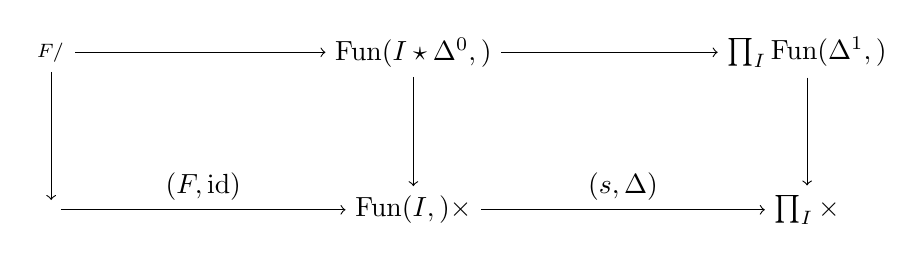
\begin{tikzpicture}
  \node (cf) at (0,0) {$\C_{F/}$};
  \node (fs) at (4.6,0) {$\mathrm{Fun}(I \star \Delta^0, \C)$};
  \node (pr) at (9.6,0) {$\prod_{I} \mathrm{Fun}(\Delta^1, \C)$};
  \node (c) at (0,-2.0) {$\C$};
  \node (fc) at (4.6,-2.0) {$\mathrm{Fun}(I, \C) \times \C$};
  \node (cc) at (9.6,-2.0) {$\prod_{I} \C \times \C$};
  \draw[->] (cf) -- (fs);
  \draw[->] (fs) -- (pr);
  \draw[->] (cf) -- (c);
  \draw[->] (fs) -- (fc);
  \draw[->] (pr) -- (cc);
  \draw[->] (c) -- node[above] {$(F, \mathrm{id})$} (fc);
  \draw[->] (fc) -- node[above] {$(s, \Delta)$} (cc);
\end{tikzpicture}
\end{center}
于是，大方块也是一个\trPullback{}。

由于\trPullback{}与任意\trProduct{}交换，我们发现存在诸\trLeftFibration{}之间的一个同构
\[
\C_{F/} \cong \prod_{I} \C^{x_i/},
\]
这就蕴含了本引理。
\end{proof}

\begin{corollary}\label{cor:horn-pushout-square}
设 $F\colon \Lambda^2_0 \to \C$ 是一个图表，描绘为
\begin{center}
\begin{tikzpicture}
  \node (x) at (0,0) {$x$};
  \node (y) at (2.2,0) {$y$};
  \node (z) at (0,-1.7) {$z$};
  \draw[->] (x) -- node[above] {$f$} (y);
  \draw[->] (x) -- node[right] {$g$} (z);
\end{tikzpicture}
\end{center}
并设 $t$ 是另一个\trObject{}。那么存在一个由∞-\trGroupoid{}组成的\trHomotopyCartesian{}%
方块
\begin{center}
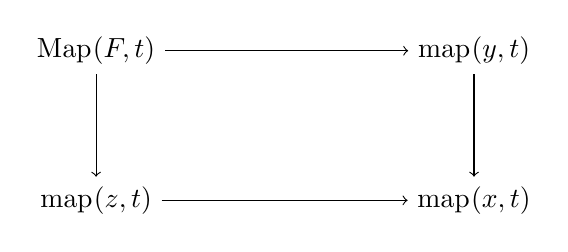
\begin{tikzpicture}
  \node (m) at (0,0) {$\mathrm{Map}_{\C}(F, t)$};
  \node (my) at (4.8,0) {$\mathrm{map}_{\C}(y, t)$};
  \node (mz) at (0,-1.9) {$\mathrm{map}_{\C}(z, t)$};
  \node (mx) at (4.8,-1.9) {$\mathrm{map}_{\C}(x, t)$};
  \draw[->] (m) -- (my);
  \draw[->] (m) -- (mz);
  \draw[->] (my) -- (mx);
  \draw[->] (mz) -- (mx);
\end{tikzpicture}
\end{center}
它在 $t$ 中是自然的。
\end{corollary}

\begin{proof}
由\cref{prop:fat-slice-pushout-cartesian}以及 $\Lambda^2_0$ 是\trPushout{}%
$\Delta^1 \amalg_{\Delta^0} \Delta^1$ 这一事实，我们发现图表
\begin{center}
\begin{tikzpicture}
  \node (f) at (0,0) {$\C^{F/}$};
  \node (ff) at (4.0,0) {$\C^{f/}$};
  \node (fg) at (0,-1.9) {$\C^{g/}$};
  \node (fx) at (4.0,-1.9) {$\C^{x/}$};
  \draw[->] (f) -- (ff);
  \draw[->] (f) -- (fg);
  \draw[->] (ff) -- (fx);
  \draw[->] (fg) -- (fx);
\end{tikzpicture}
\end{center}
既是笛卡尔又\trHomotopyCartesian{}，并且由 $\C$ 之上的诸\trLeftFibration{}组成。
此外，我们有 $\C^{f/} \simeq \C^{y/}$ 与 $\C^{g/} \simeq \C^{z/}$。过渡到一个点
$t$ 之上的\trFibre{}，我们便得到本陈述。
\end{proof}

\begin{proposition}\label{prop:pushout-colimit-existence}
设 $\C$ 是一个∞-\trCategory{}，并设 $K$ 是一个\trSimplicialSet{}，把它写成%
\trPushout{} $B \amalg_A C$，其中映射 $A \to B$ 是一个\trMonomorphism{}。设
$F\colon K \to \C$ 是一个图表。假设 $F|_B$ 容有一个\trColimit{} $y$，$F|_A$ 容有一个%
\trColimit{} $x$，而 $F|_C$ 容有一个\trColimit{}%
$z$。\footnote{译注：原书此处印作「$F|_C$ has a colimit $y$」，与下文结论「推出
$y \amalg_x z$ 是 $F$ 的一个余极限」及证明中图表 $y \leftarrow x \to z$ 相抵，应为
$z$，此处径改。——译者注}若 $\C$ 具有\trPushout{}，则一个推出 $y \amalg_x z$ 是
$F$ 的一个\trColimit{}。
\end{proposition}

\begin{proof}
下面我们将遵循 \cite{Lur09} 4.4.2.2 的论证。设 $G\colon \Lambda^2_0 \to \C$ 是由
$y \leftarrow x \to z$ 给出的图表，其中这两个映射来自
\cref{prop:induced-map-colimits}，并设
$\bar{G}\colon \Delta^1 \times \Delta^1 \to \C$ 是 $G$ 的一个\trColimit{}\trCone{}。我们
希望证明：$w = \bar{G}(1, 1)$ 是 $F\colon K \to \C$ 的一个\trColimit{}。由\cref{prop:representable-colimit}，我们必须
证明：在 $\mathrm{map}_{\C}(w, -)$ 与 $\mathrm{Map}_{\C}(F, -)$ 之间存在诸%
\trFunctor{}的一个\trEquivalence{}。用\trLeftFibration{}的语言来说，我们需要证明：
存在一个诸\trLeftFibration{}之间的\trEquivalence{} $\C^{w/} \simeq \C^{F/}$。我们有
$\C^{w/} \simeq \C^{G/}$，因为 $w$ 是 $G$ 的一个\trColimit{}。此外，存在一个%
\trHomotopyCartesian{}方块
\begin{center}
\begin{tikzpicture}
  \node (g) at (0,0) {$\C^{G/}$};
  \node (y) at (3.8,0) {$\C^{y/}$};
  \node (z) at (0,-1.9) {$\C^{z/}$};
  \node (x) at (3.8,-1.9) {$\C^{x/}$};
  \draw[->] (g) -- (y);
  \draw[->] (g) -- (z);
  \draw[->] (y) -- (x);
  \draw[->] (z) -- (x);
\end{tikzpicture}
\end{center}
由于 $x$、$y$ 与 $z$ 本身都是\trColimit{}，我们发现存在交换图表
\begin{center}
\begin{tikzpicture}
  \node (fb) at (0,0) {$\C^{F_B/}$};
  \node (fa) at (3.8,0) {$\C^{F_A/}$};
  \node (fc) at (7.6,0) {$\C^{F_C/}$};
  \node (y) at (0,-2.2) {$\C^{y/}$};
  \node (x) at (3.8,-2.2) {$\C^{x/}$};
  \node (z) at (7.6,-2.2) {$\C^{z/}$};
  \draw[->] (fb) -- (fa);
  \draw[->] (fc) -- (fa);
  \draw[->] (fb) -- node[left] {$\simeq$} (y);
  \draw[->] (fa) -- node[left] {$\simeq$} (x);
  \draw[->] (fc) -- node[left] {$\simeq$} (z);
  \draw[->] (y) -- (x);
  \draw[->] (z) -- (x);
\end{tikzpicture}
\end{center}
其中竖直的比较映射是\trJoyalEquivalence{}（见\cref{obs:induced-map-informal}）。
于是，在同伦\trPullback{}上存在一个诱导的\trEquivalence{}%
\[
\C^{G/} \simeq \C^{F/},
\]
从而 $\C^{F/}$ 的确是\trRepresentable{}，且 $w$ 是一个\trRepresentingObject{}。
\end{proof}

\begin{proposition}\label{prop:sequential-colimit}
设 $F\colon K \to \C$ 是一个\trFunctor{}，设 $K = \mathrm{colim}_{i \ge 0} K_i$ 是
一个带 $\mathbb{N}$ 标号的分解，其中每个映射 $K_i \to K_{i+1}$ 都是%
\trMonomorphism{}，并设 $F_i$ 是 $F$ 在 $K_i$ 上的限制。假设：对一切 $i$，\trFunctor{}%
$F_i$ 容许一个\trColimit{}，并且 $\C$ 容许在 $1$ 维\trSimplicialSets{}上取的%
\trColimit{}。那么 $F$ 容许一个\trColimit{}。
\end{proposition}

\begin{proof}
首先，我们发现存在诸\trLeftFibration{}之间的一个同构
$\C^{F/} \to \lim_{i \ge 0} \C^{F_i/}$，因为对每个\trSimplicialSet{} $X$，\trFunctor{}%
$X \diamond -$ 保持\trConnected{}\trColimit{}。由假设，诸 $\C^{F_i/}$ 都是%
\trCorepresented{}\trLeftFibration{}，比如说 $\C^{F_i/} \simeq \C^{x_i/}$。于是我们得到一些典范映射
$\C^{x_{i-1}/} \to \C^{x_i/}$，它们使诸比较图表交换。由\trYoneda{}引理，这些映射
全都对应于一些\trMorphism{} $\alpha_i\colon x_{i-1} \to x_i$，并且它们拼装成一个%
\trFunctor{} $G\colon I^{\infty} \to \C$。由于
$I^{\infty} = \mathrm{colim}_n I^n$，我们发现存在
$\C^{G/} \to \lim_{i \ge 0} \C^{G_i/}$。由于 $I^n$ 具有一个\trTerminalObject{}，
我们发现 $\C^{G_i/} \simeq \C^{G(i)/} = \C^{x_i/}$。\footnote{译注：原书此处印作
「$\C^{G_i} \simeq \C^{G(i)/}$」，按上下文左端应为带斜杠的\trFatSlice{}%
$\C^{G_i/}$，此处径改。——译者注}我们得到一些交换
图表
\begin{center}
\begin{tikzpicture}
  \node (fi) at (0,0) {$\C^{F_i/}$};
  \node (xi) at (4.0,0) {$\C^{x_i/}$};
  \node (gi) at (8.0,0) {$\C^{G_i/}$};
  \node (fm) at (0,-2.2) {$\C^{F_{i-1}/}$};
  \node (xm) at (4.0,-2.2) {$\C^{x_{i-1}/}$};
  \node (gm) at (8.0,-2.2) {$\C^{G_{i-1}/}$};
  \draw[->] (fi) -- (xi);
  \draw[->] (gi) -- (xi);
  \draw[->] (fi) -- (fm);
  \draw[->] (xi) -- (xm);
  \draw[->] (gi) -- (gm);
  \draw[->] (fm) -- (xm);
  \draw[->] (gm) -- (xm);
\end{tikzpicture}
\end{center}
其中所有水平映射都是\trJoyalEquivalence{}，而外侧的竖直映射都是\trIsofibration{}。
于是我们发现，在竖直极限上诱导出的映射是一个\trJoyalEquivalence{}%
$\C^{G/} \simeq \C^{F/}$。由于 $I^{\infty}$ 是 $1$ 维的，我们发现 $\C$ 容许带
$I^{\infty}$ 标号的\trColimit{}。于是 $\C^{G/}$ 是\trCorepresented{}，从而这对 $\C^{F/}$
同样成立。因此，$F$ 容许一个\trColimit{}。
\end{proof}

\begin{proposition}\label{prop:small-colimits-coproducts-pushouts}
若一个∞-\trCategory{} $\C$ 容许小\trCoproduct{}与\trPushout{}，那么它容许全部小%
\trColimit{}。
\end{proposition}

\begin{proof}
我们遵循 \cite{Lur09} 4.4.2.6 的论证。首先，我们通过对 $K$ 的维数作归纳，证明
$\C$ 容许以有限维\trSimplicialSets{} $K$ 为指标的\trColimit{}。若 $K$ 是零维的，
则它只是一个离散集合，从而其上的\trColimit{}就是\trCoproduct{}，故由假设存在。现在假设 $K$
是 $n$ 维的，并考虑它的\trSkeleton{}\trPushout{}（skeletal pushout）
\begin{center}
\begin{tikzpicture}
  \node (td) at (0,0) {$\displaystyle\coprod_{i \in I} \partial\Delta^n$};
  \node (tr) at (5.4,0) {$\mathrm{sk}_{n-1}(K)$};
  \node (bd) at (0,-2.4) {$\displaystyle\coprod_{i \in I} \Delta^n$};
  \node (br) at (5.4,-2.4) {$K$};
  \draw[->] (td) -- (tr);
  \draw[->] (td) -- (bd);
  \draw[->] (tr) -- (br);
  \draw[->] (bd) -- (br);
\end{tikzpicture}
\end{center}
对一个\trFunctor{} $F\colon K \to \C$，由\cref{prop:pushout-colimit-existence}，只需
论证 $F$ 到其余三个角中任何一个上的限制都容许一个\trColimit{}。对
$\mathrm{sk}_{n-1}(K)$ 与 $\coprod_{i \in I} \partial\Delta^n$ 而言，这由归纳假设
得出。尚待证明的是：任何\trFunctor{} $\coprod_{i \in I} \Delta^n \to \C$ 都容许一个%
\trColimit{}。由\cref{cor:diagram-simplex-limit-colimit}，我们知道每个单独的%
\trFunctor{} $\Delta^n \to \C$ 都容许一个\trColimit{}。用同样的论证，我们发现：沿
全部\trTerminalObject{}作限制给出一个\trJoyalEquivalence{}%
\[
\C^{\coprod_{i \in I} \Delta^n/} \xrightarrow{\ \simeq\ } \C^{I/},
\]
因为右零调映射的\trCoproduct{}仍是右零调的。于是，只需论证 $\C^{I/}$ 等价于一个%
\trRepresentable{}\trLeftFibration{}，这再次由 $\C$ 容许\trCoproduct{}这一假设得出。

基于这第一步，我们随后便可以利用\cref{prop:sequential-colimit}得出结论：$\C$
容许全部小\trSimplicialSets{} $K$ 的 $K$ 形状\trColimit{}，其做法是把 $K$ 写成对其
诸\trSkeleton{}取的\trColimit{}。
\end{proof}

在存在有限\trCoproduct{}的前提下，拥有\trPushout{}事实上等价于拥有\trCoequalizer{}，正如下面的
引理所揭示的。

\begin{lemma}\label{lem:pushouts-coequalizers}
若一个∞-\trCategory{} $\C$ 容许有限\trCoproduct{}，那么它容许\trPushout{}，当且仅当它容许%
\trCoequalizer{}。特别地，若 $\C$ 容许小\trCoproduct{}与\trCoequalizer{}，那么它容许全部小%
\trColimit{}。
\end{lemma}

\begin{proof}
\trCoequalizer{}范畴是图表 $\Delta^1 \leftarrow \partial\Delta^1 \to \Delta^1$ 的%
\trPushout{}。于是，由\cref{prop:pushout-colimit-existence}，若 $\C$ 容许%
\trPushout{}与有限\trCoproduct{}，则它容许\trCoequalizer{}。为了看出逆命题，人们可以类似地
循\cref{prop:pushout-colimit-existence}的思路论证。也就是说，假设 $K'$ 是%
\trSimplicialSets{}的两个\trMorphism{} $L \to K$ 的\trCoequalizer{}，并假设 $K' \to \C$
是一个\trFunctor{}，使得它到 $K$ 与到 $L$ 上的限制都容许一个\trColimit{}。那么，
诸\trColimit{}的\trCoequalizer{}就是\trFunctor{} $K' \to \C$ 的一个\trColimit{}，见
\cite{Lur09} 4.4.3.1 或\cref{ex:colimit-coequalizer}。基于这一发现，我们观察到：存在一个\trCoequalizer{}图表
\[
\Delta^0 \rightrightarrows \Delta^1 \sqcup \Delta^1
  \longrightarrow \Lambda^2_0,
\]
其中这两个映射是把顶点取为 $0$ 的那两个包含映射。由此我们可以推出：$\Lambda^2_0$
上的\trColimit{}由 $\Delta^0$ 上与 $\Delta^1 \sqcup \Delta^1$ 上取的\trColimit{}%
之间的两个映射的\trCoequalizer{}给出，而这两者均在 $\C$ 容许有限\trCoproduct{}时存在。
\end{proof}

\begin{definition}\label{def:preserve-colimit}
设 $f\colon \C \to \D$ 是∞-\trCategories{}之间的一个\trFunctor{}，并设
$F\colon K \to \C$ 是一个图表。假设 $F$ 在 $\C$ 中容许一个\trColimit{}。我们称
$f$ \emph{保持}（preserve）这个\trColimit{}，如果对某个（从而对任意）\trColimit{}\trCone{}%
$\bar{F}\colon K \star \Delta^0 \to \C$，所得图表
$K \star \Delta^0 \to \C \to \D$ 是 $fF$ 之上的一个\trColimit{}\trCone{}。此外，
我们称 $f$ 保持 $K$ 形状\trColimit{}，如果对每个容许一个\trColimit{}的\trFunctor{}%
$F\colon K \to \C$，$f$ 保持这个\trColimit{}。\footnote{译注：原书此句印作
「we say that $F$ preserves $K$-shaped colimits, if \ldots\ $F$ preserves this
colimit」，两处主语均应为 $f$（∞-范畴之间的\trFunctor{}），按印刷原样则与图表
$F$ 混淆、定义循环，此处径改。——译者注}
\end{definition}

\begin{remark}\label{rem:preserve-initial-objects}
于是，一个\trFunctor{} $f\colon \C \to \D$ 保持 $K$ 形状\trColimit{}，如果对每个%
\trFunctor{} $F\colon K \to \C$，诱导\trFunctor{} $\C^{F/} \to \D^{fF/}$ 保持%
\trInitialObject{}。
\end{remark}

\begin{proposition}\label{prop:preserve-small-colimits}
设 $F\colon \C \to \D$ 是∞-\trCategories{}之间的一个\trFunctor{}。那么，$F$ 保持
小\trColimit{}，当且仅当它保持小\trCoproduct{}与\trPushout{}。若把\trPushout{}换成%
\trCoequalizer{}，同样的结论也成立。
\end{proposition}

\begin{proof}
\cref{ex:preserves-small-colimits}。
\end{proof}

我们将不加证明地汇集\trColimit{}的下列性质（但我们建议读者尝试把其中一些当作
练习来证明）。

\begin{proposition}\label{prop:fun-preserve-colimits}
若 $\D$ 是（余）\trComplete{}且 $K$ 是一个小\trSimplicialSet{}，那么
$\mathrm{Fun}(K, \D)$ 仍是（余）\trComplete{}，并且诸\trColimit{}被\trPointwise{}计算。
换言之，对 $K$ 的每个\trObject{} $x$，求值\trFunctor{}%
$\mathrm{Fun}(K, \D) \to \D$ 保持（余）\trLimit{}。
\end{proposition}

\begin{proposition}\label{prop:fat-slice-preserve-colimits}
设 $\C$ 是一个（余）\trComplete{}∞-\trCategory{}，并设 $F\colon K \to \C$ 是一个
图表。那么 $\C^{/F}$ 容许诸\trColimit{}，且\trFunctor{} $\C^{/F} \to \C$ 保持诸%
\trColimit{}。对偶地，$\C^{F/}$ 容许诸\trLimit{}，且 $\C^{F/} \to \C$ 保持诸%
\trLimit{}。
\end{proposition}

\begin{proof}
\cite{Lur09} 1.2.13.8。
\end{proof}

\begin{proposition}\label{prop:fat-slice-cocomplete}
设 $\C$ 是一个\trCocomplete{}∞-\trCategory{}，并设 $F\colon K \to \C$ 是一个图表。那么
$\C^{F/}$ 仍是\trCocomplete{}。对偶地，若 $\C$ 是\trComplete{}，则 $\C^{/F}$ 是%
\trComplete{}。然而，这些\trForgetfulFunctor{}一般并不保持这些（余）\trLimit{}。
\end{proposition}

\begin{proposition}\label{prop:left-fibration-preserve-colimits}
设 $f\colon \E \to \C$ 是一个\trLeftFibration{}，并设 $K$ 是一个\trWeaklyContractible{}%
\trSimplicialSet{}。那么 $f$ 保持 $K$ 形状\trColimit{}。同样地，诸%
\trRightFibration{}保持\trContractible{}\trLimit{}。
\end{proposition}

\begin{proof}
\cite{Lur09} 4.4.2.8 与 4.4.2.9。
\end{proof}

对下述定理，我们稍后会给出一个利用\trStraightening{}--\trUnstraightening{}%
\trEquivalence{}的独立证明。然而，下面的证明有一个优点：我们能够看到\trLimit{}与%
\trColimit{}如所预期地被给出。

\begin{theorem}\label{thm:cat-infinity-spc-bicomplete}
∞-\trCategories{} $\mathrm{Cat}_{\infty}$ 与 $\mathrm{Spc}$ 容许全部小\trLimit{}%
与\trColimit{}。
\end{theorem}

\begin{proof}
由\cref{prop:small-colimits-coproducts-pushouts}，只需证明这些∞-\trCategories{}%
容许小\trProduct{}、\trCoproduct{}、\trPullback{}与\trPushout{}。正如我们先前已经看到的，\trCoproduct{}与\trProduct{}相当
容易。我们来证明 $\mathrm{Cat}_{\infty}$ 容许\trPullback{}；其余各种情形在风格上
都是类似的。为此，考虑一个图表 $F\colon \Lambda^2_2 \to \mathrm{Cat}_{\infty}$，它由
两个\trFunctor{}%
\[
\D \xrightarrow{\ p\ } \C \xleftarrow{\ f\ } \C'
\]
给出。不失一般性，我们可以假设 $\D \to \C$ 是一个\trIsofibration{}。我们令 $\D'$
为上述\trSimplicialSets{}图表的\trPullback{}，并令
$\bar{F}\colon \Delta^1 \times \Delta^1 \to \mathrm{Cat}_{\infty}$ 为整个%
\trPullback{}图表。我们希望证明：$\mathrm{Cat}_{\infty}^{/F}$ 是一个%
\trRepresentable{}\trRightFibration{}。由\cref{cor:horn-pushout-square}的对偶论证，我们知道存在一个
既笛卡尔又\trHomotopyCartesian{}方块
\begin{center}
\begin{tikzpicture}
  \node (cf) at (0,0) {$\mathrm{Cat}_{\infty}^{/F}$};
  \node (ff) at (5.0,0) {$\mathrm{Cat}_{\infty}^{/f}$};
  \node (pc) at (0,-2.2) {$\mathrm{Cat}_{\infty}^{/p}$};
  \node (cc) at (5.0,-2.2) {$\mathrm{Cat}_{\infty}^{/\C}$};
  \draw[->] (cf) -- (ff);
  \draw[->] (cf) -- (pc);
  \draw[->] (ff) -- (cc);
  \draw[->] (pc) -- (cc);
\end{tikzpicture}
\end{center}
此外，存在一个典范映射
$\mathrm{Cat}_{\infty}^{/\D'} \simeq \mathrm{Cat}_{\infty}^{/\bar{F}} \to \mathrm{Cat}_{\infty}^{/F}$，
而我们希望证明这个\trFunctor{}是一个\trEquivalence{}。我们将证明它%
\trEssentiallySurjective{}且\trFullyFaithful{}。至于本质满性：
$\mathrm{Cat}_{\infty}^{/F}$ 的一个\trObject{}可以（在相差一个\trEquivalence{}的
意义下）由∞-\trCategories{}的一个交换图表
\footnote{译注：原书此处印作「an object of $\C^{/F}$」，但本证明中
$F\colon \Lambda^2_2 \to \mathrm{Cat}_{\infty}$ 并非 $\C$ 中的图表，按上下文应为
$\mathrm{Cat}_{\infty}^{/F}$，此处径改。——译者注}
\begin{center}
\begin{tikzpicture}
  \node (e) at (0,0) {$\E$};
  \node (d) at (3.4,0) {$\D$};
  \node (cp) at (0,-2.0) {$\C'$};
  \node (c) at (3.4,-2.0) {$\C$};
  \draw[->] (e) -- (d);
  \draw[->] (e) -- (cp);
  \draw[->] (d) -- node[right] {$p$} (c);
  \draw[->] (cp) -- node[above] {$f$} (c);
\end{tikzpicture}
\end{center}
来表示。由\trPullback{} $\D'$ 的\trUniversalProperty{}，$\E$ 带有到 $\D'$ 的一个
唯一映射，而这个映射给出了 $\mathrm{Cat}_{\infty}^{/\D'}$ 中所得的\trObject{}。
为了看出全忠实性，只需证明：对 $\mathrm{Cat}_{\infty}^{/\D'}$ 的任意两个%
\trObject{} $\E, \E'$，下述\trMappingSpace{}图表是\trHomotopyCartesian{}：
\begin{center}
\begin{tikzpicture}
  \node (a) at (0,0)
    {$\mathrm{map}_{\mathrm{Cat}_{\infty}^{/\D'}}(\E, \E')$};
  \node (b) at (7.6,0)
    {$\mathrm{map}_{\mathrm{Cat}_{\infty}^{/\C'}}(\E, \E')$};
  \node (c) at (0,-2.4)
    {$\mathrm{map}_{\mathrm{Cat}_{\infty}^{/\D}}(\E, \E')$};
  \node (d) at (7.6,-2.4)
    {$\mathrm{map}_{\mathrm{Cat}_{\infty}^{/\C}}(\E, \E')$};
  \draw[->] (a) -- (b);
  \draw[->] (a) -- (c);
  \draw[->] (b) -- (d);
  \draw[->] (c) -- (d);
\end{tikzpicture}
\end{center}
但这由\trSliceCategory{}中诸\trMappingSpace{}的一个描述、第 3 章中的%
\cref{prop:mapping-space-slice}、$\D' \cong \D \times_{\C} \C'$ 这一事实以及
$\D \to \C$ 是一个\trIsofibration{}这一事实得出。
\end{proof}
